% This file was created by tikzplotlib v0.9.1.
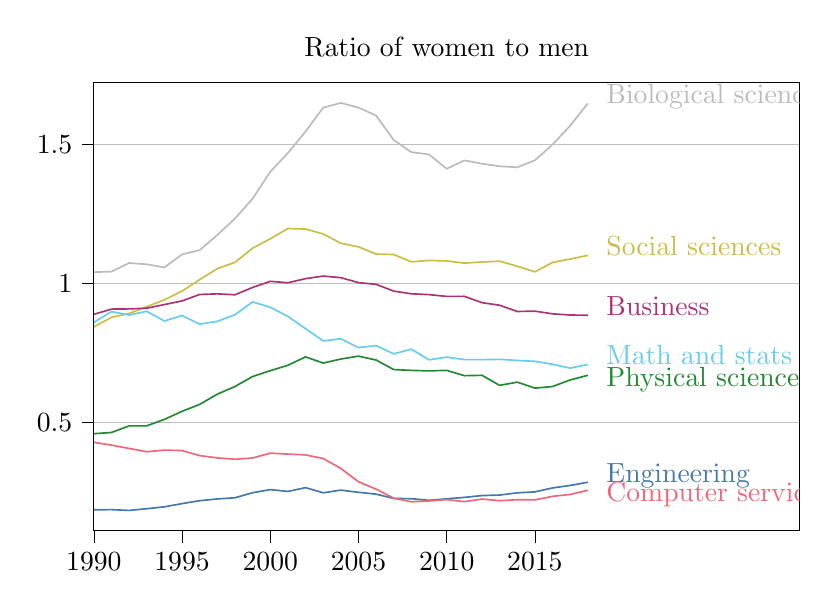
\begin{tikzpicture}

\definecolor{color0}{rgb}{0.266666666666667,0.466666666666667,0.666666666666667}
\definecolor{color1}{rgb}{0.933333333333333,0.4,0.466666666666667}
\definecolor{color2}{rgb}{0.133333333333333,0.533333333333333,0.2}
\definecolor{color3}{rgb}{0.8,0.733333333333333,0.266666666666667}
\definecolor{color4}{rgb}{0.4,0.8,0.933333333333333}
\definecolor{color5}{rgb}{0.666666666666667,0.2,0.466666666666667}

\begin{axis}[
height=207pt,
tick align=outside,
tick pos=left,
title={Ratio of women to men},
width=300pt,
x grid style={white!69.0196078431373!black},
xmin=1990, xmax=2030,
xtick style={color=black},
xtick={1990,1995,2000,2005,2010,2015},
xticklabels={\(\displaystyle 1990\),\(\displaystyle 1995\),\(\displaystyle 2000\),\(\displaystyle 2005\),\(\displaystyle 2010\),\(\displaystyle 2015\)},
ymajorgrids,
ymin=0.111868877532793, ymax=1.72181142557414,
ytick style={color=black}
]
\addplot [semithick, color0]
table {%
1990 0.187528491020203
1991 0.187889814376831
1992 0.18504810333252
1993 0.191165328025818
1994 0.198027372360229
1995 0.209525942802429
1996 0.219993829727173
1997 0.226323843002319
1998 0.230563402175903
1999 0.248593807220459
2000 0.259858369827271
2001 0.253314614295959
2002 0.266838073730469
2003 0.248422026634216
2004 0.258007287979126
2005 0.250089168548584
2006 0.243573904037476
2007 0.228035092353821
2008 0.227158188819885
2009 0.221451997756958
2011 0.231951236724854
2012 0.238436937332153
2013 0.240317106246948
2014 0.248236060142517
2015 0.251599311828613
2016 0.265729546546936
2017 0.274784326553345
2018 0.286244869232178
};
\addplot [semithick, color1]
table {%
1990 0.429780006408691
1991 0.419558525085449
1993 0.395862579345703
1994 0.4017493724823
1995 0.399999976158142
1996 0.381898045539856
1997 0.373727560043335
1998 0.368845701217651
1999 0.373373627662659
2000 0.390813827514648
2001 0.387295722961426
2002 0.384417414665222
2003 0.37157928943634
2004 0.335911631584167
2005 0.288139462471008
2006 0.261456251144409
2007 0.22909951210022
2008 0.216255187988281
2009 0.219069957733154
2010 0.223915338516235
2011 0.216599345207214
2012 0.225852251052856
2013 0.219969153404236
2014 0.223478555679321
2015 0.222921013832092
2016 0.235600471496582
2017 0.242461562156677
2018 0.257417798042297
};
\addplot [semithick, color2]
table {%
1990 0.460548996925354
1991 0.464974999427795
1992 0.4886314868927
1993 0.488829135894775
1994 0.512030601501465
1995 0.540966749191284
1996 0.565948724746704
1997 0.602615833282471
1998 0.629949331283569
1999 0.666009306907654
2000 0.686820149421692
2001 0.706353425979614
2002 0.736422896385193
2003 0.7142094373703
2004 0.72872519493103
2005 0.739134073257446
2006 0.725082635879517
2007 0.690871238708496
2008 0.687974691390991
2009 0.686181664466858
2010 0.688009262084961
2011 0.668954968452454
2012 0.67028284072876
2013 0.634251594543457
2014 0.645684003829956
2015 0.62436580657959
2016 0.629948854446411
2017 0.653665065765381
2018 0.67027759552002
};
\addplot [semithick, color3]
table {%
1990 0.843912363052368
1991 0.878591060638428
1992 0.892377018928528
1993 0.916429758071899
1994 0.941344499588013
1995 0.972469568252563
1996 1.01399052143097
1997 1.05340433120728
1998 1.07601177692413
1999 1.12696635723114
2000 1.16036009788513
2001 1.19738638401031
2002 1.19550442695618
2003 1.1779510974884
2004 1.14445388317108
2005 1.13158094882965
2006 1.10574865341187
2007 1.10396230220795
2008 1.07783782482147
2009 1.08280813694
2010 1.08092784881592
2011 1.07324647903442
2012 1.07712745666504
2013 1.0801340341568
2014 1.06191837787628
2015 1.04196679592133
2016 1.07565009593964
2017 1.0877937078476
2018 1.10102880001068
};
\addplot [semithick, color4]
table {%
1990 0.86025857925415
1991 0.899104356765747
1992 0.886856079101562
1993 0.900158047676086
1994 0.865336656570435
1995 0.88508152961731
1996 0.85411524772644
1997 0.864051580429077
1998 0.88809061050415
1999 0.93377161026001
2000 0.914776563644409
2001 0.881730198860168
2003 0.793915510177612
2004 0.801473140716553
2005 0.769950985908508
2006 0.776896238327026
2007 0.747289896011353
2008 0.764146089553833
2009 0.725896239280701
2010 0.73568868637085
2011 0.726636171340942
2012 0.726435899734497
2013 0.727647542953491
2014 0.723636150360107
2015 0.720515251159668
2016 0.709809184074402
2017 0.696071982383728
2018 0.709341764450073
};
\addplot [semithick, color5]
table {%
1990 0.889276146888733
1991 0.908068180084229
1992 0.908786058425903
1993 0.911298394203186
1995 0.937413215637207
1996 0.960581421852112
1997 0.962796211242676
1998 0.959450006484985
1999 0.985843420028687
2000 1.00777983665466
2001 1.00261080265045
2002 1.01744496822357
2003 1.02670252323151
2004 1.02088141441345
2005 1.00308656692505
2006 0.996885895729065
2007 0.972628951072693
2008 0.96298623085022
2009 0.959978342056274
2010 0.95364236831665
2011 0.953920364379883
2012 0.931203603744507
2013 0.921860694885254
2014 0.899493217468262
2015 0.900677680969238
2016 0.891088247299194
2017 0.886778354644775
2018 0.88598895072937
};
\addplot [semithick, white!73.3333333333333!black]
table {%
1990 1.04078304767609
1991 1.04256737232208
1992 1.07366561889648
1993 1.06894600391388
1994 1.05757308006287
1995 1.10440194606781
1996 1.11996006965637
1997 1.17428719997406
1998 1.23312425613403
1999 1.30454993247986
2000 1.40134906768799
2001 1.46844744682312
2002 1.54577028751373
2003 1.63139522075653
2004 1.64863216876984
2005 1.63168549537659
2006 1.602987408638
2007 1.51491057872772
2008 1.47168242931366
2009 1.46346211433411
2010 1.41208970546722
2011 1.44205784797668
2012 1.42999362945557
2013 1.42106962203979
2014 1.41722071170807
2015 1.44253933429718
2016 1.49894797801971
2017 1.56678104400635
2018 1.64683747291565
};
\draw (axis cs:2018.5,0.286244813278008) node[
  anchor=base west,
  text=color0,
  rotate=0.0
]{Engineering};
\draw (axis cs:2018.5,0.217417838961352) node[
  anchor=base west,
  text=color1,
  rotate=0.0
]{Computer services};
\draw (axis cs:2018.5,0.63027762382224) node[
  anchor=base west,
  text=color2,
  rotate=0.0
]{Physical sciences};
\draw (axis cs:2018.5,1.10102875591671) node[
  anchor=base west,
  text=color3,
  rotate=0.0
]{Social sciences};
\draw (axis cs:2018.5,0.709341764874964) node[
  anchor=base west,
  text=color4,
  rotate=0.0
]{Math and stats};
\draw (axis cs:2018.5,0.885989010989011) node[
  anchor=base west,
  text=color5,
  rotate=0.0
]{Business};
\draw (axis cs:2018.5,1.64683752645192) node[
  anchor=base west,
  text=white!73.3333333333333!black,
  rotate=0.0
]{Biological sciences};
\end{axis}

\end{tikzpicture}
